
\chapter{Software Quality Assurance}

This chapter describes the processes used during the development and deployment of the Consolidated Fire and Smoke Transport model (CFAST).  This software quality assurance (SQA) plan is intended to guide the planning for modifications to the model, provide required reviews for both software and associated documentation of the model, define testing to be conducted prior to the release of an updated model, describe problem reporting and resolution procedures, and ensure all records, source code, and released software is kept available for the life of the code.  While this memorandum and many of our practices follow the Institute of Electrical and Electronics Engineers (IEEE) standard for software quality assurance, IEEE 730-2002 \cite{IEEE:730}, other standards have been followed as well.  Most notably, ASTM 1355-05, �Standard Guide for Evaluating the Predictive Capability of Deterministic Fire Models� \cite{ASTM:E1355} has been used extensively to guide the documentation, verification, and validation of the model.

CFAST is intended for use only by those competent in the field of fire safety and is intended only to supplement the informed judgment of the qualified user. The software package is a computer model which has limitations based on the way it is used, and the data used for calculations. All results should be evaluated by a qualified user.

The SQA process and requirements outlined in this chapter apply specifically to the CFAST and is focused on ensuring the quality of the numerical predictions of the model.  The user interface that may be used to develop input for the model is included in this process to insure that changes to the model are reflected in the user interface and in the data files created by the user interface for use by the model.  Of course, users must ensure that the input files developed for the simulations accurately reflect the desired model inputs, whether developed using the supplied user interface, another third-party interface, or manually input with a spreadsheet or text editor program.  Documentation of these inputs is included as part of the model documentation outlined below.

\section{Relevant Publications}

To accompany the model and simplify its use, NIST has developed a Technical Reference Guide \cite{CFAST_Tech_Guide_6} and a User's Guide \cite{CFAST_Users_Guide_6} and this Software and Validation Guide.  The Technical Reference Guide describes the underlying physical principles and summarizes sensitivity analysis, model validation, and model limitations consistent with ASTM E 1355 \cite{ASTM:E1355}.  The User�s Guide describes how to use the model.  

The U.S. Nuclear Regulatory Commission has published a verification and validation study of five selected fire models commonly used in support of risk-informed and performance-based fire protection at nuclear power plants \cite{NRCNUREG1824_CFAST}. In addition to an extensive study of the CFAST model, the report compares the output of several other models ranging from simple hand calculations to more complex CFD codes such as the Fire Dynamics Simulator (FDS) developed by NIST.

While this document and many of our practices make extensive use of ASTM 1355, �Standard Guide for Evaluating the Predictive Capability of Deterministic Fire Models� \cite{ASTM:E1355} to guide the documentation, verification, and validation of the model, other standards have been followed as well.  Most notably, our software quality assurance processes were guided by the IEEE standard for software quality assurance, IEEE 730-2002 \cite{IEEE:730}.

In addition, numerous related documents available at http://cfast.nist.gov provide a wealth of information concerning including earlier versions of the model and its user interface. Software quality assurance (SQA) plan is intended to guide the planning for modifications to the model, provide required reviews for both software and associated documentation of the model, define testing to be conducted prior to the release of an updated model, describe problem reporting and resolution procedures, and ensure all records, source code, and ensure released software is kept available for the life of the code.  

\section{Model Management}

CFAST is developed and maintained by the Building and Fire Research Laboratory (BFRL) at the National Institute of Standards and Technology (NIST). Like all projects at BFRL, a designated project leader is responsible for directing and prioritizing model development, error correction, and preparation of documentation for the model development.  The organization chart in Figure \ref{figOrgChart} provides a graphical representation of the software quality organization structure for CFAST

\begin{figure}
\begin{center}
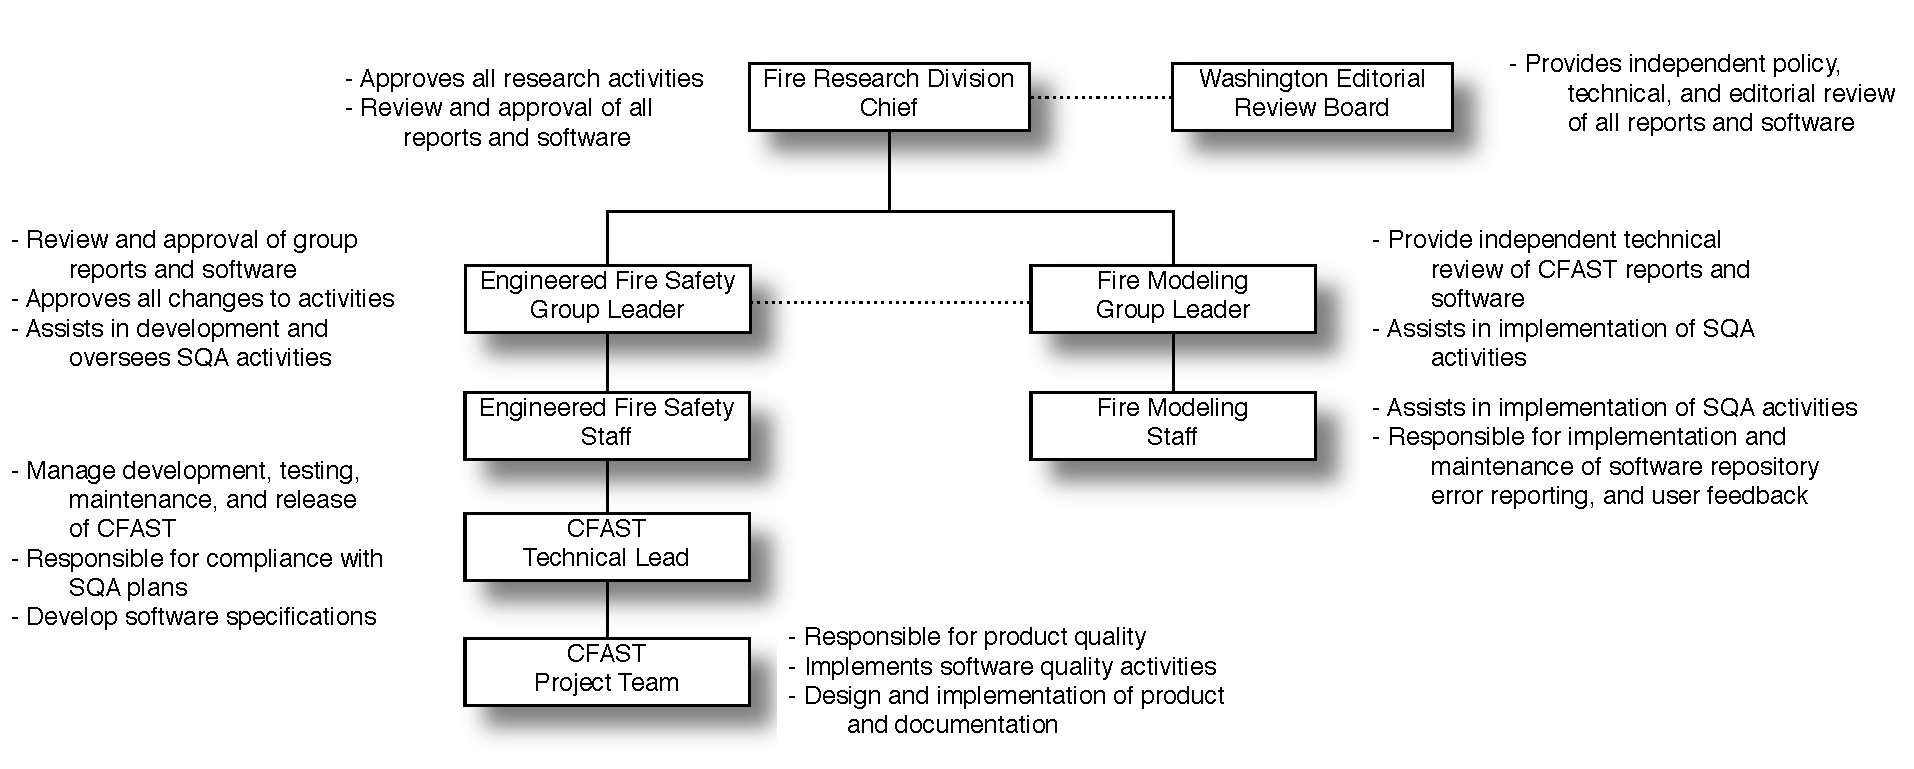
\includegraphics[width=6.5in]{FIGURES/OrgChart.pdf}\\
\end{center}
\caption{CFAST SQA Organization Structure.}
 \label{figOrgChart}
\end{figure}

Review and approval of software and documentation is part of the standard review process for any report or other product developed by NIST. A minimum of five reviews are required prior to release of reports or software, including two independent technical peer reviews, two technical and management reviews at the technical workgroup and division level, and a policy review at the NIST-wide level.  This review is documented and recorded on the NIST standard form NIST 114 along with official approval notification provided to the primary author of the product.

CFAST is distributed exclusively through a NIST website dedicated to the CFAST model (http://cfast.nist.gov).  Content of the website is the responsibility of the CFAST project leader and the BFRL webmaster. Additions and changes to the website are made only with the approval of the CFAST project leader after any required NIST reviews.

\section{SQA Documentation}

The released version of CFAST is documented by three primary publications, the Technical Reference Guide\cite{CFAST_Tech_Guide_6}, the User�s Guide \cite{CFAST_Users_Guide_6}, and this Software and Model Evaluation Guide. The documents apply to the newest version of the model available on the NIST website. The Technical Reference Guide describes the underlying physical principles, provides a review of model verification and validation efforts by NIST and others, and describes the limitations of the model.  The User's Guide describes how to use the model, includes a detailed description of the model inputs and outputs, and provides a process to ensure the correct installation of the model. There are also documents archived on the website that are applicable to older versions of both the model and user interface.

During development of new or corrected features for the model, the following documents are developed:

\begin{itemize}
\item {\em Software Requirements and Design Specifications:}  This is an internal memorandum that documents the intended function of a new or enhanced feature, describes its implementation in sufficient detail to allow an independent review of the feature, and identifies any new or existing testing and validation required prior to acceptance of the feature in a release version of the model.  This document forms the basis for necessary changes to the technical reference guide and user�s guide for the model once the new feature is ready for general release. As defined in IEEE 730-2002 \cite{IEEE:730}, this document includes the software requirements specification, software design description, and software verification and validation plan. The level of detail in this document depends on the complexity of the change to the model. 

\item {\em Software Validation and Testing Results:}  This is an internal memorandum that demonstrates the use of the new feature through appropriate test cases and describes validation and verification tests performed to ensure the new feature is implemented properly without unexpected changes in other features. This document forms the basis for the model verification and validation documentation included as part of this Software and Experimental Validation guide. As defined in IEEE 730-2002 \cite{IEEE:730}, this document includes the software verification and validation report. The level of detail in this document depends on the complexity of the change to the model.
\end{itemize}

Both of these documents are reviewed internally to NIST by group staff not directly involved with model development. In addition, the NIST review process documents the review and approval of released versions of the model as described above.

Source code for released versions of the model is maintained with version control software that allows tracking of specific changes to the model from version to version.   Each version of the model released includes a unique version number that identifies the major and minor version numbers of the release as well as the date of release. Differences with prior versions are documented and provided as part of the release and on the CFAST website so that users can ascertain what effect these changes will have on prior calculations.

\section{Standards, Practices, Conventions, and Metrics}

Prior to final implementation of a new feature or change, a review of the proposed modification is conducted by a developer who is not involved in the modification.  This review includes review and concurrence of the software requirements and design specification as well as more detailed review of code changes as the complexity of the modification requires. Review and acceptance of the software requirements and design specification by interested project sponsors or users may be included as appropriate. Name and date of approval and/or review is noted electronically in the document.

Review of the testing and validation report is also conducted by a developer who is not involved in the modification prior to proposed model release. Any significant changes in model output (typically a change greater than 1 \% of a given output) should be explained based on changes to the code as a result of a new feature.  Name and date of approval and/or review is noted electronically in the document.

\section{Software Reviews}

Software reviews are outlined as part of the standard practices described above.  The standard NIST review process includes review of software and documentation prior to any report or product release by NIST.

\section{Model Testing}

Individual testing of model algorithms are made by the developers during any revision of the model. Often, this testing forms the basis for any new standard test cases included with future model releases. System release testing of the model prior to release includes the following:

\begin{itemize}
\item Examination of results of test cases specific to any model modifications made as appropriate.  Comparison with analytic solutions to simplified problems is desirable when available.

\item Examination of results of standard test cases included with the release version of the model. Any changes in the output from prior versions is explained (and documented in the software testing and validation results report) by modifications made to the model.

\item For major new releases of the model, a complete suite of test cases should be compared to those from previous versions of the model.  At a minimum this includes the set of validation exercises described in NUREG 1824 \cite{NRCNUREG1824}, but may include additional example cases or validation exercises as appropriate.
\end{itemize}

\section{Problem Reporting and Resolution}

NIST maintains an e-mail address specifically for inquiries and problem reporting for the CFAST model (cfast@nist.gov).  These e-mails are directed to the CFAST project leader for response and resolution as appropriate.  Inquiries and responses are catalogued and retained by the project leader.

NIST has developed an automated reporting and resolution tracking website for use with the CFAST model to facilitate tracking and cataloging of inquires, problems, and model enhancements / revisions. This is included as part of the CFAST website at http://cfast.nist.gov

\section{Tools, Techniques, and Methodologies}

NIST will use an automated comparison tool (under development) to compare CFAST predictions between different versions of the model and with experimental data to simplify testing and validation for the CFAST model.

\section{Media Control}

Release versions of the CFAST model are available exclusively on the CFAST specific website maintained by the Building and Fire Research Laboratory (BFRL) at NIST. This website is included in NIST�s automated backup and recovery system for computer systems organization wide.

Development versions of the model are maintained by the CFAST project leader.  All software and documents are included in NIST�s automated backup and recovery system for computer systems organization wide.

Both of these computer systems are available only to specified personnel, including the CFAST project leader and BFRL webmaster.

\section{Supplier Control}

CFAST is entirely a product of BFRL / NIST and as such does not include any commercial software libraries. The differential equation solver used by CFAST, DASSL, is a publicly available software package.  Full source code for the solver as used by CFAST is maintained under version control with the rest of the model code.

BFRL currently uses Microsoft Visual Studio 2005 and Intel Visual Fortran 10.1 for development\footnote{Certain commercial entities, equipment, or materials may be identified in this document 
in order to describe an experimental procedure or concept adequately. Such identification 
is not intended to imply recommendation or endorsement by the National Institute of 
Standards and Technology, nor is it intended to imply that the entities, materials, or 
equipment are necessarily the best available for the purpose.}.  Prior to any change to a different development system, a full test suite of test cases must be compared to verify consistent operation of the model and model results.

\section{Records Collection, Maintenance, and Retention}

All software, documentation, and SQA documents are retained by the CFAST project leader, typically in electronic form. Software and documentation is also maintained and archived on the NIST CFAST website as part of the version control software for the model. 

BFRL management approval is required prior to destruction of old or out-of-date records. Records are typically maintained for a minimum of 25 years.

\section{Training}

No specific training is identified for use of this SQAP.  Details of training requirements for use of the model included in the CFAST user�s guide is applicable to developers of the model as well.

{\section{Risk Management}

The primary risk management tool for software developed and released by NIST is the official NIST review process for software, documents, and other products of NIST. Official approval is required prior to release of the model for general use.

